\begin{tikzpicture}
  \node[inner sep=0] (torusfield) {%
    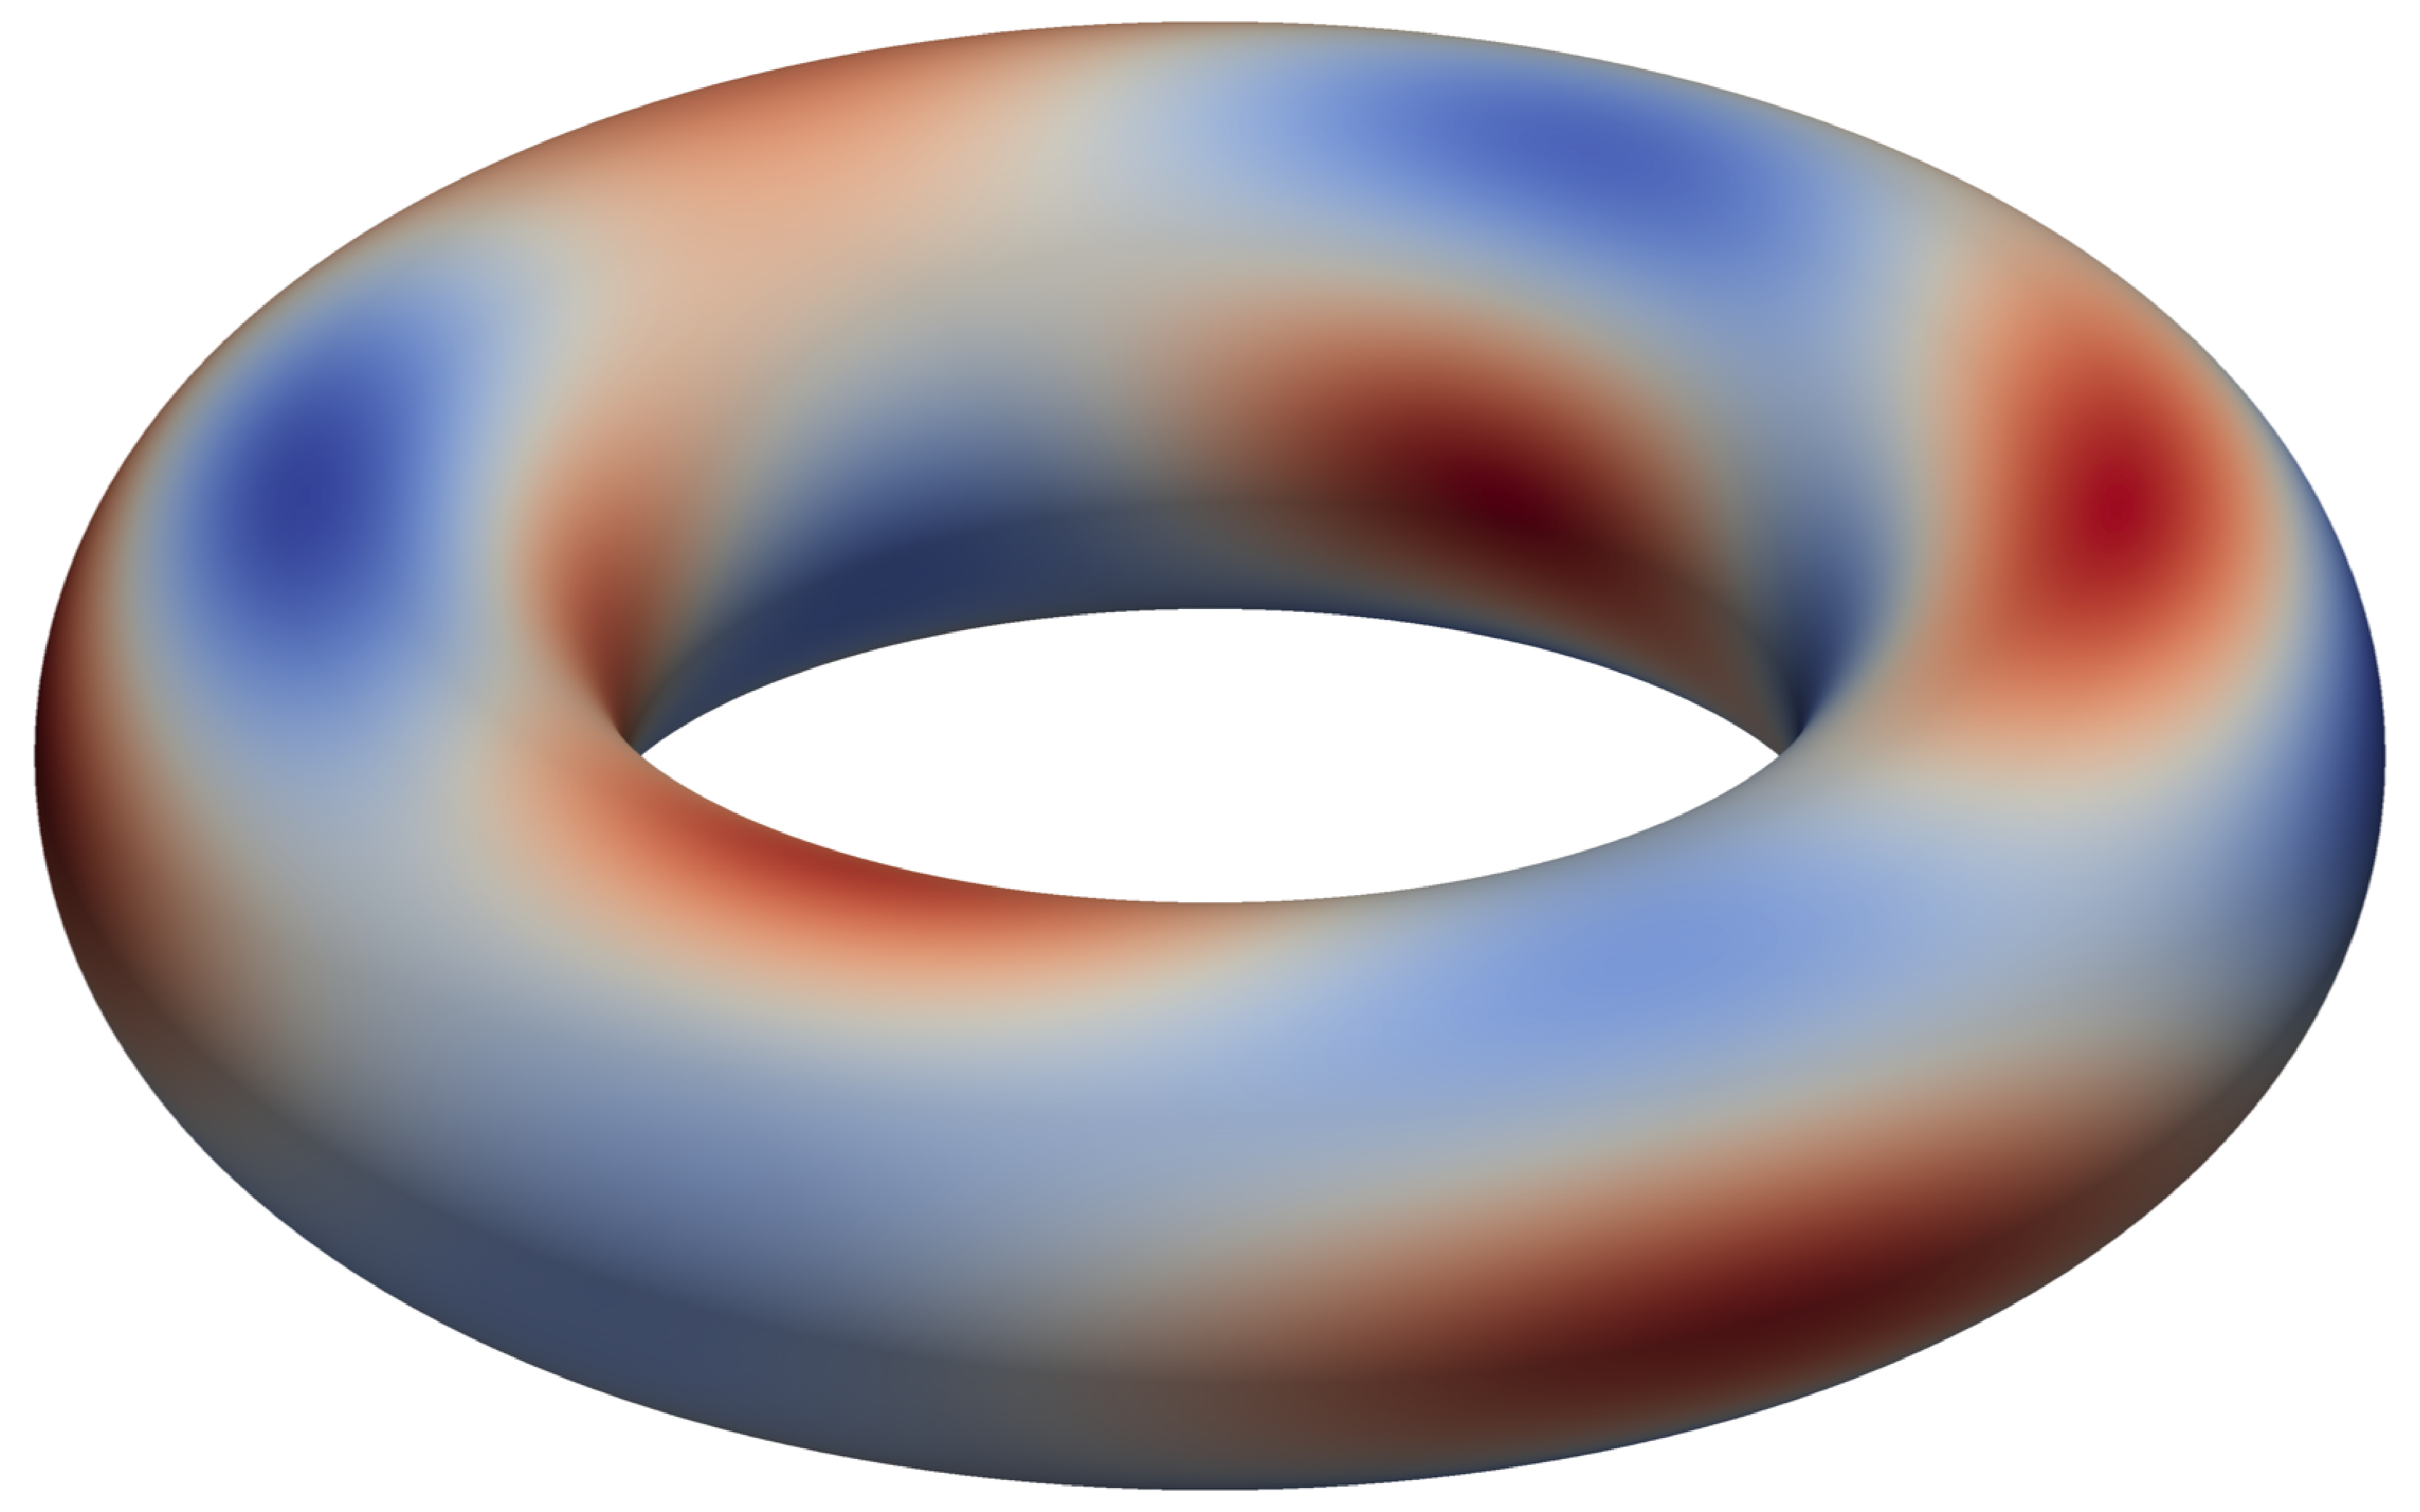
\includegraphics[width=0.7\textwidth]{img/torus_ddfv_field.pdf}%
  };

  \path let \p1=(torusfield.south west), \p2=(torusfield.north west) in
    \pgfextra{\xdef\torusfieldheight{\the\dimexpr\y2-\y1\relax}};
  \pgfplotscolorbardrawstandalone[
    % Approximation de la palette Matplotlib ``coolwarm'', échantillonnée directement dans celle qu'utilise le script PyVista.
    colormap={coolwarm}{[1cm]
      rgb255(0cm)=(59,76,192)
      rgb255(1cm)=(98,130,234)
      rgb255(2cm)=(141,176,254)
      rgb255(3cm)=(185,208,249)
      rgb255(4cm)=(221,220,220)
      rgb255(5cm)=(245,196,172)
      rgb255(6cm)=(244,152,122)
      rgb255(7cm)=(221,95,75)
      rgb255(8cm)=(180,4,38)
    },
    colorbar left,
    point meta min=-1,
    point meta max=1,
    parent axis height=\torusfieldheight,
    colorbar style={
      at={(torusfield.west)},
      anchor=east,
      height=0.5*\torusfieldheight,
      width=5pt,
      ytick={0},
      ylabel={$u$},
    },
  ]
\end{tikzpicture}
